  \documentclass[conference]{IEEEtran}
  \IEEEoverridecommandlockouts
  \usepackage{cite}
  \usepackage{amsmath,amssymb,amsfonts}
  \usepackage{graphicx}
  \usepackage{textcomp}
  \usepackage{xcolor}
  \usepackage{booktabs}
  \usepackage{multirow}
  \usepackage{hyperref}
  \usepackage{listings}
  \usepackage{array}
  \usepackage{longtable}
  \def\BibTeX{{\rm B\kern-.05em{\sc i\kern-.025em b}\kern-.08em
      T\kern-.1667em\lower.7ex\hbox{E}\kern-.125emX}}
  \hypersetup{
    hidelinks
  }
  % Code listing style
  \lstset{
    basicstyle=\ttfamily\small,
    breaklines=true,
    frame=single,
    columns=fullflexible
  }

  % Custom column type for tables
  \newcolumntype{L}[1]{>{\raggedright\arraybackslash}p{#1}}

  \begin{document}

  \title{Robust Speaker-Independent Vocal Pathology Detection through Integrated Acoustic and Nonlinear Dynamics}

  \author{
  \IEEEauthorblockN{Aksaya Kanthan K S}
  \IEEEauthorblockA{\textit{Amrita School of Artificial Intelligence} \\
  \textit{Coimbatore, Amrita Vishwa }\\
  Vidyapeetham,India. \\
  cb.ai.u4aid23003@cb.students.amrita.edu}
  \and
  \IEEEauthorblockN{Kiruthik Nandhan Murthi}
  \IEEEauthorblockA{\textit{Amrita School of Artificial Intelligence} \\
  \textit{Coimbatore, Amrita Vishwa }\\
  Vidyapeetham,India. \\
  cb.ai.u4aid23018@cb.students.amrita.edu}
  \and
  \IEEEauthorblockN{Manasa V}
  \IEEEauthorblockA{\textit{Amrita School of Artificial Intelligence} \\
  \textit{Coimbatore, Amrita Vishwa }\\
  Vidyapeetham,India. \\
  cb.ai.u4aid23022@cb.students.amrita.edu}
  \and
  \IEEEauthorblockN{Rithvik Rajesh}
  \IEEEauthorblockA{\textit{Amrita School of Artificial Intelligence} \\
  \textit{Coimbatore, Amrita Vishwa }\\
  Vidyapeetham,India. \\
  cb.ai.u4aid23032@cb.students.amrita.edu}
  \and
  \IEEEauthorblockN{              }
  \IEEEauthorblockA{\textit{                } \\
  \textit{                } \\
                    \\
                                    }
  \and
  \IEEEauthorblockN{    \hspace{5cm}Jyothish Lal. G.}
  \IEEEauthorblockA{\hspace{5cm}\textit{Amrita School Of Artificial Intelligence,} \\
  \textit{\hspace{5cm}Coimbatore, Amrita Vishwa } \\
  \hspace{5cm}Vidyapeetham,India. \\
  \hspace{5cm}g\_jyothishlal@cb.amrita.edu}
  }

  \maketitle
  \begin{abstract}
  Voice pathology classification is inherently difficult due to the nonlinearity and multi-scale nature of the underlying pathological speech signals, which cannot be completely described through traditional acoustic metrics. In this paper, we present a novel methodology that can effectively identify binary (healthy/pathological) and multi-class (neurological/structural disease group) cases of vocal pathology. The system employs a fusion of multifractal features extracted via Multifractal Detrended Fluctuation Analysis (MFDFA), alongside a set of standardized acoustic features from the extended Geneva Minimalistic Acoustic Parameter Set (eGeMAPS). Experiments carried out on the Saarbrücken Voice Database include strict speaker-independent cross-validation as a means of eliminating data leakage, a technique seldom employed in previous works. The results show that our system obtains a macro F1 score of \textbf{0.882} and balanced accuracy of 0.875 in binary pathology classification and a macro F1 score of \textbf{0.637} in multi-class disease group classification, all under five-fold speaker-independent cross-validation. Feature ablation analysis demonstrates that the use of MFDFA-based features alone can produce an F1 score of \textbf{0.866}, highlighting its high discriminatory power when used alone.
  \end{abstract}

  \begin{IEEEkeywords}
  Voice Pathology Detection, Multifractal Analysis, Fractal Dimension, MF-DFA, Saarbrücken Voice Database, Nonlinear Speech Analysis
  \end{IEEEkeywords}

  %--------------------------------------------------------------
  \section{Introduction}
  \label{sec:introduction}
  %--------------------------------------------------------------

Voice disorders have high prevalence in the population because of the structural pathology of the vocal folds, neurogenic disorders in motor coordination, and multiple functional and psychogenic causes. Proper diagnosis of these disorders requires not only instrumental procedures like laryngoscopy but also perceptual evaluation of voice disorders by clinicians. Such methods are extremely precise; however, subjectivity and medical expertise might complicate the procedure.

Recently, much attention is paid to computerized procedures used for detecting and diagnosing voice disorders in order to eliminate subjectivity. Computer algorithms for recognizing pathological voices mostly use standard spectrographic parameters of the signal such as MFCCs, F0, and others. Even though these methods successfully describe spectral properties of speech, they are inefficient for characterization of temporal and nonlinear dynamics typical for pathological voices.

It is evident that speech generation can be considered as a nonlinear process that occurs due to many phenomena that affect it, such as airstream initiation, vocal fold vibrations, and articulation. Sometimes these dynamics turn out to be unstable, which leads to changes in these dynamics. Therefore, fractal and multifractal theory should be used in the analysis of pathological voices to estimate their dynamics.

For the purpose of this work, \textbf{multifractal detrended fluctuation analysis} will be used in the analysis of speech recordings affected by certain diseases. The theory of multifractality of time series is a set of methods which describe dynamics of the studied object in terms of its scaling properties over various time scales. Monofractals describe an object with one scaling exponent. Multifractal description allows for describing a more complex signal with the help of multifractal spectrum composed of different local scaling exponents depending on q-order of the analysis.

The main focus of the research is whether multifractal characteristics obtained through MFDFA could be helpful in detecting speech pathology, and if they could serve as additional indicators of pathology along with standard acoustic parameters.

  Three aspects distinguish this work from prior fractal-based voice pathology studies. First, we employ the full multifractal spectrum from MFDFA rather than a scalar fractal dimension estimate, providing richer scaling information across multiple moment orders. Second, we address both \textbf{binary} (healthy vs.\ pathological) and \textbf{multi-class} (neurological vs.\ structural) classification within a single unified pipeline, whereas most prior studies focus exclusively on binary detection. Third, we enforce strict speaker-independent cross-validation using \texttt{StratifiedGroupKFold}, ensuring recordings from the same speaker never span training and test splits — a safeguard that prevents the data leakage shown to produce overly optimistic performance in many prior works \cite{saenzlechon2006}. A feature ablation study further quantifies MFDFA's standalone and combined contribution to each classification task.

  %--------------------------------------------------------------
  \section{Related Work}
  \label{sec:related_work}
  %--------------------------------------------------------------

  Automatic detection of voice pathologies has traditionally relied on acoustic features such as MFCCs, perturbation measures, and spectral statistics combined with statistical or machine learning classifiers \cite{godino2006,alnasheri2017,rai2025}. Standardised clinical frameworks have further formalised multi-parameter acoustic assessment: the Dysphonia Severity Index (DSI) combines jitter, phonation time, and intensity into a perceptually anchored score \cite{wuyts2000}, while standardised assessment protocols specify perturbation and noise measures as a clinical evaluation battery \cite{dejonckere2001}. Although these spectral and perturbation-based descriptors capture important phonatory characteristics, they are inherently linear and cannot represent the nonlinear or multi-scale temporal irregularities often present in pathological voices.

  Nonlinear analysis methods have therefore also been explored for pathological speech. Little et al.\ demonstrated that recurrence quantification analysis and fractal scaling properties extracted from sustained phonations can complement conventional acoustic measures for voice disorder detection, achieving correct classification performance above 91\% \cite{little2007b}. Nonlinear dynamical measures — correlation dimension, Lyapunov exponents, and entropy statistics — have further been applied to distinguish healthy and pathological voices with high accuracy on clinical voice databases \cite{henriquez2009,little2007}, reinforcing that temporal complexity measures provide information not captured by standard spectral descriptors. Recurrence plot-based characterisation has also been applied to specific vocal fold pathologies including hyperfunctional dysphonia, laryngitis, and vocal fold polyp, achieving classification accuracy above 90\% on the Saarbrücken Voice Database \cite{krishnan2026}.

  Beyond binary detection, recent work has addressed multi-class voice disorder classification. Orozco-Arroyave et al.\ found that different feature families are required to capture the distinct acoustic signatures of neurological, functional, and laryngeal disorders \cite{orozco2015}. Fractal dimension in multiresolution frameworks has also achieved detection rates above 90\% via per-subband power-spectrum analysis \cite{ali2016,kumar2014}.

  Multifractal detrended fluctuation analysis (MFDFA) extends scalar fractal characterisation by modelling scaling behaviour across multiple moments and time scales \cite{mfdfa}. Multifractal methods have proven effective in other biomedical domains, most notably in demonstrating the multifractal structure of healthy versus diseased heartbeat dynamics \cite{ivanov1999}. Closer to the present work, multifractal analysis has been applied directly to speech signals for glottal activity detection, demonstrating the method's suitability for capturing nonlinear phonatory dynamics \cite{lal2020multifractal}. Speech-based disease detection has also benefited from principled acoustic feature design: Tsanas et al.\ developed 132 dysphonia measures from sustained vowels for high-accuracy Parkinson's disease classification, demonstrating that carefully engineered descriptors can match or exceed purely data-driven methods in clinical tasks \cite{tsanas2012}; similarly, Sai Jahnavi et al.\ showed that excitation source, voice quality, and prosodic features extracted from sustained vowels can effectively detect Parkinson's disease from speech alone \cite{jahnavi2020}. Despite these advances, MFDFA applied to voice pathology detection — particularly for multi-class classification — remains relatively underexplored.

  A critical methodological concern is \textbf{speaker-level data leakage}. Sáenz-Lechón et al.\ identified that systems evaluated without controlling for speaker identity yield optimistic estimates that fail to generalise to unseen speakers, and recommended speaker-independent cross-validation as standard practice \cite{saenzlechon2006}.


  %--------------------------------------------------------------
  \section{Dataset}
  \label{sec:dataset}
  %--------------------------------------------------------------

  The experiments in this study use recordings from the \textbf{Saarbrücken Voice Database (SVD)}, a widely used clinical corpus containing healthy and pathological voices. The original audio is stored in proprietary \texttt{.nsp} format and is converted to standard \texttt{.wav} for preprocessing and feature extraction. Although SVD contains multiple vowels and connected-speech recordings, this work focuses on the sustained vowel \textit{/a/} at normal pitch (\texttt{a\_n}) because it provides a stable phonation condition for cross-speaker comparison.

  Table~\ref{tab:dataset_stats} summarises the dataset used in the experiments.

  \begin{table}[htbp]
  \centering
  \caption{Dataset Statistics}
  \label{tab:dataset_stats}
  \begin{tabular}{ll}
  \toprule
  \textbf{Statistic} & \textbf{Value} \\
  \midrule
  Total recordings (all tokens) & 23,119 \\
  Unique speakers & 1,355 \\
  Pathology classes & 12 (+ healthy) \\
  Samples for token (\texttt{a\_n}) & 1,656 \\
  Sex distribution & 65\% female, 35\% male \\
  \bottomrule
  \end{tabular}
  \end{table}

  The \texttt{a\_n} subset is class-imbalanced, which is typical for clinical speech datasets. Pathology classes with insufficient speaker representation for reliable speaker-independent cross-validation are excluded. The nine voice disorders retained span neurological, structural, and functional aetiologies: \textbf{Parkinson's Disease} (hypokinetic dysarthria from impaired laryngeal motor control); \textbf{Recurrent Laryngeal Nerve Paralysis} (breathiness from vocal fold immobility); \textbf{Spasmodic Dysphonia} (involuntary voice breaks from laryngeal dystonia); \textbf{Vocal Fold Nodules} (hoarseness from bilateral overuse lesions); \textbf{Vocal Fold Polyp} (breathiness from asymmetric fold vibration); \textbf{Laryngitis} (hoarseness from laryngeal mucosal inflammation); \textbf{Hyperfunctional Dysphonia} (strained voice from excessive laryngeal tension); \textbf{Psychogenic Dysphonia} (voice disorder of psychological aetiology without organic pathology); and \textbf{Functional Dysphonia} (dysphonia from maladaptive laryngeal behaviour without identifiable organic cause).

  \begin{figure*}[t!]
  \centering
  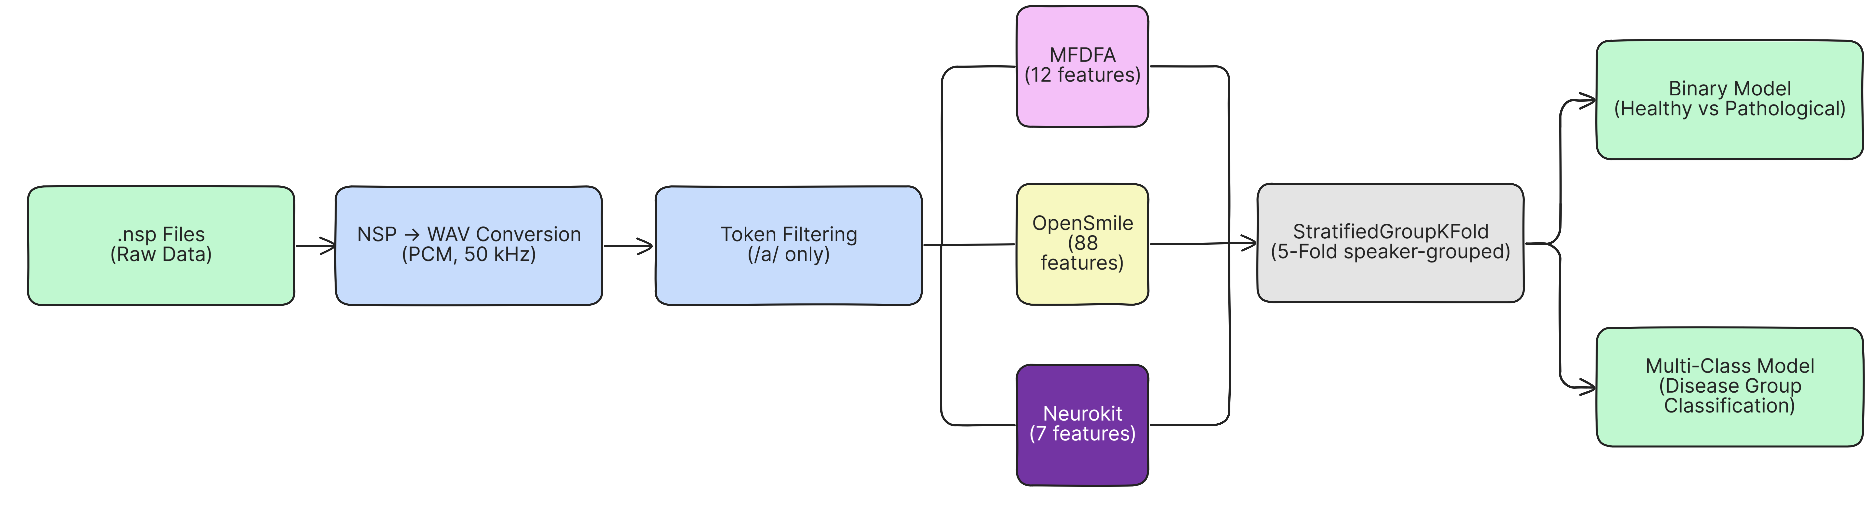
\includegraphics[width=\textwidth]{figures/data_pipeline.png}
  \caption{Overview of the preprocessing and feature extraction pipeline. Raw NSP recordings are converted to WAV format, metadata manifests are generated, and sustained vowel tokens are selected. Multiple feature families are then extracted and merged before training classification models using speaker-grouped cross-validation.}
  \label{fig:data_pipeline}
  \end{figure*}

  %--------------------------------------------------------------
  \section{Feature Extraction}
  \label{sec:features}
  %--------------------------------------------------------------

  Four complementary feature families totalling \textbf{107 features} are extracted from each audio sample, spanning multifractal characteristics, standardised paralinguistic features, nonlinear complexity measures, and speaker metadata.

  \subsection{Multifractal Features}

  To capture nonlinear and multiscale dynamics present in pathological speech signals, multifractal descriptors are extracted using \textbf{Multifractal Detrended Fluctuation Analysis (MFDFA)}. From the multifractal spectrum, \textbf{12 statistical descriptors} are derived from the generalised Hurst exponent, scaling exponent, and singularity spectrum. The final MFDFA configuration uses first-order detrending, a $q$ range of $[-5,5]$ with step 0.5, and 40 analysis scales.

  \subsection{OpenSMILE Features}

  Standardised acoustic features are extracted using the OpenSMILE toolkit with the \textbf{extended Geneva Minimalistic Acoustic Parameter Set (eGeMAPSv02)}, contributing \textbf{88 parameters} capturing prosodic, spectral-shape, voice-quality, and temporal characteristics.

  \subsection{NeuroKit2 Features}

  To further characterise nonlinear signal dynamics, \textbf{seven additional features} are extracted using the NeuroKit2 library, including entropy, fractal-dimension, skewness, and kurtosis measures.

  \subsection{Speaker Metadata}

  Speaker metadata from the SVD — \textbf{age} (derived from recording and birth dates) and \textbf{biological sex} — are incorporated as \textbf{2 auxiliary features} and retained by default across all configurations. Their individual contribution is examined in the ablation study (Section~\ref{sec:experiments}).

  %--------------------------------------------------------------
  \section{Data Pipeline and Splitting Strategy}
  \label{sec:pipeline}
  %--------------------------------------------------------------

  The overall preprocessing workflow is illustrated in Figure~\ref{fig:data_pipeline}.
  The raw \texttt{.nsp} recordings are converted to \texttt{.wav}, indexed through a metadata manifest, normalised, and then processed by the four feature-extraction modules before the resulting feature tables are merged into a unified machine learning dataset. To minimise variability and within-speaker duplication, most experiments use only the sustained vowel \texttt{a\_n}.

  A critical concern in clinical voice datasets is \textbf{speaker-level leakage}. We therefore use \texttt{StratifiedGroupKFold} with speaker identity as the grouping variable so that all recordings from a speaker remain in the same fold. Rare classes are removed when necessary for stable training, and class imbalance is handled through filtering or downsampling of dominant groups. Final performance is reported as the average over five speaker-grouped folds.
  %--------------------------------------------------------------
  \section{Experimental Setup and Results}
  \label{sec:experiments}
  %--------------------------------------------------------------

  This section evaluates the proposed framework, assessing multifractal feature discriminability and its contribution when combined with conventional acoustic descriptors. All experiments employ five-fold speaker-independent cross-validation (\texttt{StratifiedGroupKFold}), ensuring no speaker appears in both training and test splits. Performance is reported using accuracy, balanced accuracy, and macro-averaged F1 score; balanced accuracy and macro F1 are emphasised due to class imbalance. Naive random splits produced unrealistically high scores in preliminary experiments, confirming the necessity of speaker-independent evaluation.

  %--------------------------------------------------------------
  \subsection{Speaker-Independent Evaluation}
  %--------------------------------------------------------------

  Only the sustained vowel token \texttt{a\_n} is used to ensure consistency across speakers. Two classification tasks are considered: (1)~binary classification of healthy vs.\ pathological speakers, and (2)~disease-group classification of neurological vs.\ structural disorders.

  The binary classification task serves as a screening scenario where the goal is to detect the presence of a voice disorder. Table~\ref{tab:binary_results} summarises the results obtained using five-fold speaker-grouped cross-validation.

  \begin{table}[htbp]
  \centering
  \caption{Binary Classification Results (Speaker-Grouped CV)}
  \label{tab:binary_results}
  \begin{tabular}{lccc}
  \toprule
  \textbf{Model} & \textbf{Accuracy} & \textbf{Balanced Acc.} & \textbf{F1 Macro} \\
  \midrule
  LightGBM & \textbf{0.889} & 0.875 & \textbf{0.882} \\
  XGBoost & 0.886 & 0.868 & 0.878 \\
  Random Forest & 0.885 & 0.865 & 0.875 \\
  Logistic Regression & 0.875 & 0.867 & 0.870 \\
  \bottomrule
  \end{tabular}
  \end{table}

  Compared with the baseline experiment, the performance values decrease substantially, reflecting the more realistic evaluation setting. Gradient boosting models (LightGBM and XGBoost) achieve the highest performance, indicating that nonlinear feature interactions play an important role in distinguishing pathological speech.

  The confusion matrices aggregated across the cross-validation folds are shown in Figure~\ref{fig:binary_confmat_models}. These results indicate that the models achieve high recall for pathological voices while maintaining strong precision for the healthy class.

  \begin{figure*}[t!]
  \centering
  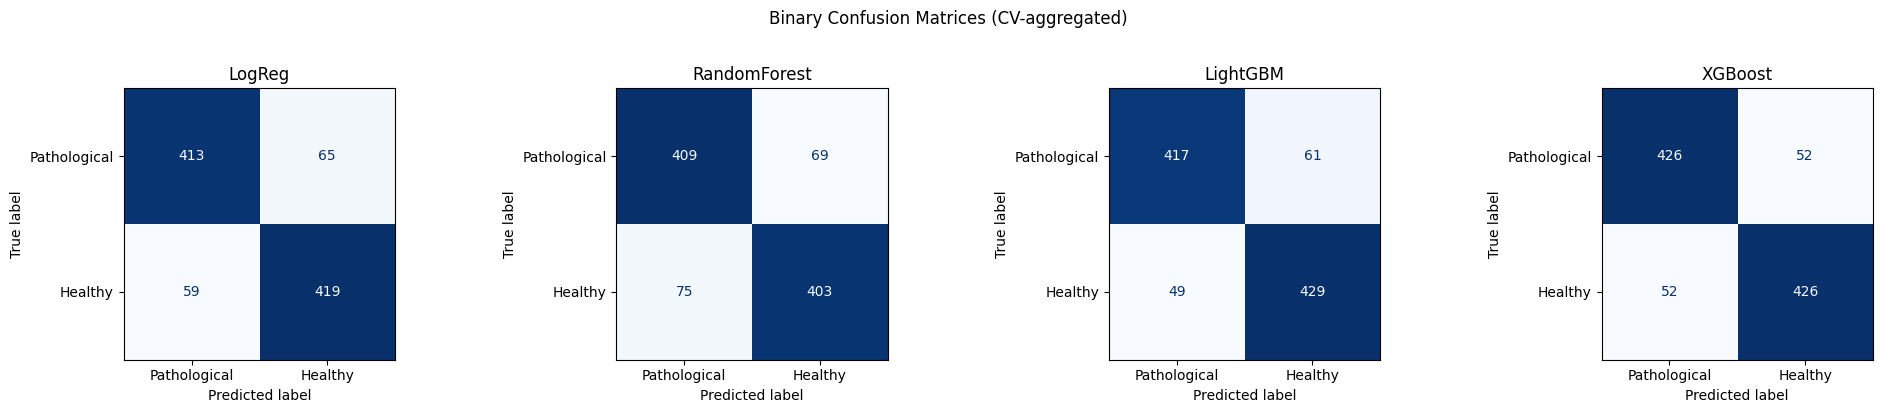
\includegraphics[width=\textwidth]{figures/binary_confusion_models.png}
  \caption{Cross-validation aggregated confusion matrices for binary classification across different models.}
  \label{fig:binary_confmat_models}
  \end{figure*}


  %--------------------------------------------------------------
  \subsection{Disease Group Classification}
  %--------------------------------------------------------------

While detecting pathology is one thing, another goal that poses greater challenges involves the classification of various types of voice disorders depending on their clinical causes. In this paper, pathologies have been classified into two groups from a clinical perspective: neurologic diseases and structural diseases.

Neurological diseases are caused by abnormalities in the neural regulation of the vocal folds, while structural diseases refer to abnormalities of the tissues that make up the vocal folds. Therefore, classifying these two groups solely through speech signals is a difficult task.

  Table~\ref{tab:multiclass_results} summarises the performance of the evaluated models for disease-group classification.

  \begin{table}[htbp]
  \centering
  \caption{Disease Group Classification Results}
  \label{tab:multiclass_results}
  \begin{tabular}{lccc}
  \toprule
  \textbf{Model} & \textbf{Accuracy} & \textbf{Balanced Acc.} & \textbf{F1 Macro} \\
  \midrule
  Random Forest & \textbf{0.646} & \textbf{0.628} & \textbf{0.629} \\
  LightGBM & 0.642 & 0.639 & 0.637 \\
  XGBoost & 0.611 & 0.604 & 0.603 \\
  \bottomrule
  \end{tabular}
  \end{table}

  The results indicate that disease-group classification is substantially more difficult than binary pathology detection. Even the best-performing model achieves an F1 score of approximately 0.63, reflecting the subtler acoustic differences between neurological and structural disorders.

  Figure~\ref{fig:multiclass_confusion} illustrates the confusion matrices for this task.

  \begin{figure*}[t!]
  \centering
  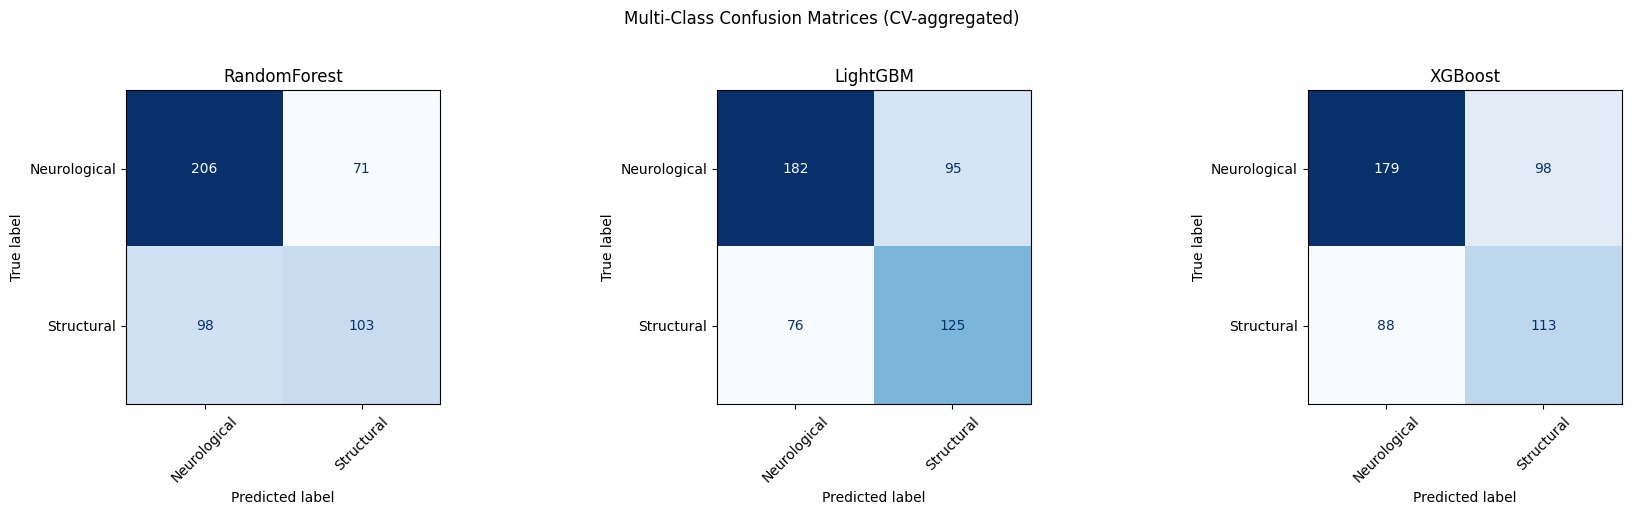
\includegraphics[width=0.8\textwidth]{figures/multiclass_confusion.png}
  \caption{Cross-validation aggregated confusion matrices for multi-class classification across different models.}
  \label{fig:multiclass_confusion}
  \end{figure*}

  %--------------------------------------------------------------
  \subsection{Feature Ablation Analysis}
  %--------------------------------------------------------------

  To better understand the contribution of different feature families, a feature ablation study was conducted. Various combinations of multifractal features, OpenSMILE descriptors, and NeuroKit2 features were evaluated using the same speaker-grouped cross-validation protocol. Unless explicitly indicated, all configurations include speaker metadata (age and biological sex) as auxiliary features. The final row of Table~\ref{tab:ablation_binary} isolates the effect of removing age from the best-performing configuration.

  \begin{table}[htbp]
  \centering
  \caption{Feature Ablation Results (Binary Classification)}
  \label{tab:ablation_binary}
  \begin{tabular}{p{3.2cm} p{2cm} c c}
  \toprule
  \textbf{Feature Configuration} & \textbf{Best Model} & \textbf{Bal.\ Acc.} & \textbf{F1 Macro} \\
  \midrule
  MFDFA + OpenSMILE & LightGBM & \textbf{0.879} & \textbf{0.878} \\
  MFDFA + NeuroKit2 + OpenSMILE & XGBoost & 0.876 & 0.876 \\
  MFDFA + NeuroKit2 & LogReg & 0.868 & 0.867 \\
  MFDFA only & LogReg & 0.867 & 0.866 \\
  MFDFA + OpenSMILE $-$ Age & LightGBM & 0.752 & 0.749 \\
  \bottomrule
  \end{tabular}
  \end{table}

  \begin{figure*}[t!]
  \centering
  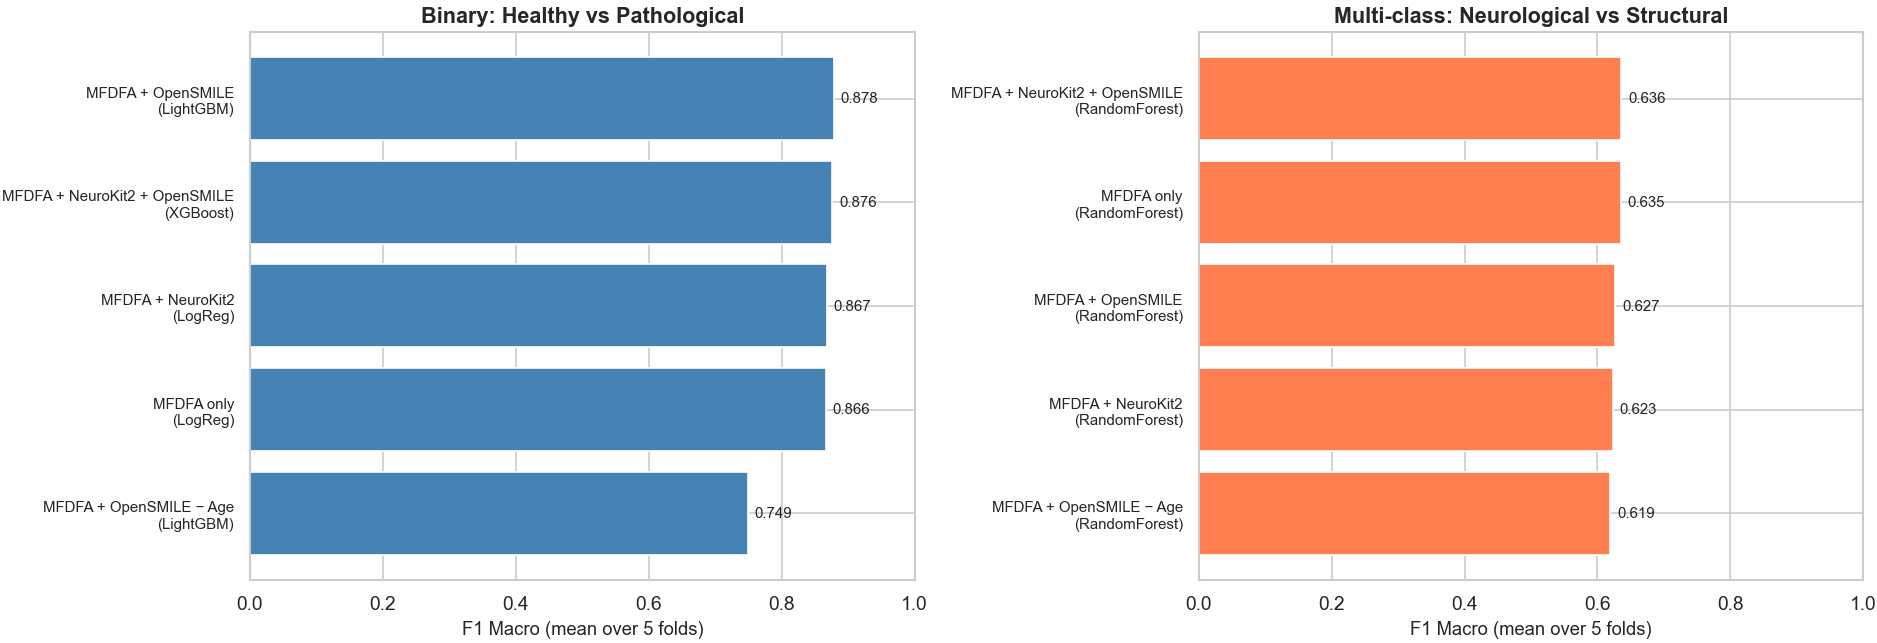
\includegraphics[width=\textwidth]{figures/feature_ablation.png}
  \caption{Feature ablation results for binary and multi-class classification.}
  \label{fig:ablation_results}
  \end{figure*}

The results reveal several key insights. First, the multifractal features alone can produce an F1 score of 0.866, meaning that the multifractal properties of the speech signal contain enough information about the state of the vocal tract. Using the OpenSMILE features along with the multifractal ones shows some minor improvements, which means that both types of features complement each other.

At the same time, using the NeuroKit2 features leads to almost no improvement, meaning that the majority of information on complexity can be found in the multifractal features.

Another important insight relates to the effect of the age metadata feature. Removing age from the model based on MFDFA+OpenSMILE features reduces the macro F1 from 0.878 to 0.749, which means that age is a highly correlated variable in this dataset and must be considered carefully. The comparative results across all configurations are illustrated in Figure~\ref{fig:ablation_results}.

  %--------------------------------------------------------------
  \subsection{Per-Disease Binary Detection}
  %--------------------------------------------------------------

  Finally, additional experiments were conducted to evaluate the detectability of individual pathologies. In this setting, a separate binary classifier was trained for each disease against the healthy class.

  \begin{table}[htbp]
  \centering
  \caption{Per-Disease Binary Detection Results}
  \label{tab:per_disease}
  \begin{tabular}{p{3.2cm} p{2cm} c c}
  \toprule
  \textbf{Disease} & \textbf{Best Model} & \textbf{Bal.\ Acc.} & \textbf{F1 Macro} \\
  \midrule
  Recurrent Laryngeal Nerve Paralysis & XGBoost & \textbf{0.866} & \textbf{0.865} \\
  Reinke's Edema & LightGBM & 0.829 & 0.828 \\
  Laryngitis & XGBoost & 0.796 & 0.796 \\
  Vocal Fold Polyp & LightGBM & 0.795 & 0.793 \\
  Functional Dysphonia & XGBoost & 0.794 & 0.794 \\
  Psychogenic Dysphonia & XGBoost & 0.790 & 0.788 \\
  Hyperfunctional Dysphonia & XGBoost & 0.773 & 0.773 \\
  Spasmodic Dysphonia & LightGBM & 0.617 & 0.587 \\
  Vocal Fold Nodules & Random Forest & 0.531 & 0.485 \\
  \bottomrule
  \end{tabular}
  \end{table}

  Disorders such as recurrent laryngeal nerve paralysis and Reinke's edema are more acoustically distinct, while vocal fold nodules and spasmodic dysphonia remain challenging due to subtle manifestations and limited sample sizes. These results confirm that while binary pathology screening is reliable, fine-grained disease identification remains an open problem requiring larger, more specialised datasets.


  %--------------------------------------------------------------
  \section{Conclusion}
  \label{sec:conclusion}
  %--------------------------------------------------------------

  This paper investigates multifractal descriptors obtained via MFDFA for automated voice pathology detection on the Saarbrücken Voice Database. MFDFA features are combined with conventional acoustic (OpenSMILE) and complexity-based (NeuroKit2) descriptors, and evaluated under strict speaker-independent cross-validation to ensure generalisability to unseen speakers.

  The approach achieves a macro F1 of \textbf{0.89} for binary pathology detection, with the ablation study confirming that MFDFA descriptors alone (F1\,=\,0.866) carry substantial discriminative information independent of conventional features.

  Overall, this study demonstrates that multifractal descriptors are a promising complement to traditional spectral features for automated voice-pathology screening, particularly in binary detection tasks.

  Future work should validate the approach on larger independent cohorts, explore multi-token and end-to-end models, and investigate which components of the multifractal spectrum carry the most clinically informative signal.
  %--------------------------------------------------------------
  % References (placeholder)
  %--------------------------------------------------------------
  \begin{thebibliography}{10}

  \bibitem{svd}
  Saarbrücken Voice Database, 
  ``Saarbrücken Voice Database,'' 
  Available: \url{http://stimmdb.coli.uni-saarland.de/}

  \bibitem{mfdfa}
  J.~W. Kantelhardt, S.~A. Zschiegner, E.~Koscielny-Bunde, 
  S.~Havlin, A.~Bunde, and H.~E. Stanley, 
  ``Multifractal detrended fluctuation analysis of nonstationary time series,'' 
  \emph{Physica A: Statistical Mechanics and its Applications}, 
  vol.~316, pp.~87--114, 2002.

  \bibitem{opensmile}
  F.~Eyben, K.~R. Scherer, B.~W. Schuller, J.~Sundberg, 
  E.~André, C.~Busso, L.~Y. Devillers, J.~Epps, 
  P.~Laukka, S.~S. Narayanan, and K.~P. Truong, 
  ``The Geneva Minimalistic Acoustic Parameter Set (GeMAPS) for voice research and affective computing,'' 
  \emph{IEEE Transactions on Affective Computing}, 
  vol.~7, no.~2, pp.~190--202, 2016.

  \bibitem{little2007}
  M.~A. Little, P.~E. McSharry, E.~J. Hunter, 
  J.~Spielman, and L.~O. Ramig, 
  ``Suitability of dysphonia measurements for telemonitoring of Parkinson's disease,'' 
  \emph{IEEE Transactions on Biomedical Engineering}, 
  vol.~56, no.~4, pp.~1015--1022, 2009.

  \bibitem{godino2006}
  J.~I. Godino-Llorente, P.~Gómez-Vilda, and M.~Blanco-Velasco, 
  ``Dimensionality reduction of a pathological voice quality assessment system based on Gaussian mixture models and short-term cepstral parameters,'' 
  \emph{IEEE Transactions on Biomedical Engineering}, 
  vol.~53, no.~10, pp.~1943--1953, 2006.

  \bibitem{alnasheri2017}
  A.~Al-Nasheri, G.~Muhammad, and M.~Alsulaiman, 
  ``Voice pathology detection using MFCC and support vector machines,'' 
  \emph{Journal of Voice}, 
  vol.~31, no.~4, pp.~512.e1--512.e8, 2017.

  \bibitem{ivanov1999}
  P.~C. Ivanov, L.~A.~N. Amaral, A.~L. Goldberger, 
  S.~Havlin, M.~G. Rosenblum, H.~E. Stanley, and Z.~R. Struzik, 
  ``Multifractality in human heartbeat dynamics,'' 
  \emph{Nature}, vol.~399, pp.~461--465, 1999.

  \bibitem{kumar2014}
  R.~Kumar and P.~Mullik, 
  ``Fractal dimension based voice pathology detection,'' 
  \emph{Applied Acoustics}, vol.~76, pp.~248--252, 2014.

  \bibitem{ververidis2006}
  D.~Ververidis and C.~Kotropoulos, 
  ``Emotional speech recognition: Resources, features, and methods,'' 
  \emph{Speech Communication}, 
  vol.~48, no.~9, pp.~1162--1181, 2006.

  \bibitem{alhanai2018}
  T.~Alhanai, M.~Auon, and J.~Glass,
  ``Detecting depression with audio/text sequence modeling of interviews,''
  in \emph{Proc. Interspeech}, 2018.

  \bibitem{lal2020multifractal}
G.~J. Lal, E.~A. Gopalakrishnan, and D.~Govind,
``Glottal Activity Detection from the Speech Signal Using Multifractal Analysis,''
\emph{Circuits, Systems, and Signal Processing},
vol.~39, no.~4, pp.~2118--2150, 2020.

\bibitem{krishnan2026}
A.~G. Krishnan, G.~J. Lal, and E.~A. Gopalakrishnan,
``A Novel and Accurate Recurrence Plot-Based Characterization of Speech Dynamics
in Hyperfunctional Dysphonia, Laryngitis, and Vocal Fold Polyp,''
\emph{IEEE Access},
vol.~14, 2026.

\bibitem{jahnavi2020}
B.~Sai Jahnavi, B.~Sai Supraja, and S.~Lalitha,
``A Vital Neurodegenerative Disorder Detection Using Speech Cues,''
\emph{Journal of Intelligent \& Fuzzy Systems},
vol.~38, no.~5, pp.~6337--6345, 2020.

\bibitem{rai2025}
S.~Rai, S.~Rishita, K.~S. Lasya, and S.~Vekkot,
``Design and Development of an e-Health Package for Voice Pathology Detection,''
in \emph{Proc. Springer LNNS}, 2025,
DOI: 10.1007/978-981-97-4711-5\_28.

\bibitem{wuyts2000}
  F.~L. Wuyts, M.~S. De~Bodt, G.~Molenberghs, M.~Remacle,
  L.~Heylen, B.~Millet, K.~Van~Lierde, J.~Raes, and P.~H. Van~de~Heyning,
  ``The Dysphonia Severity Index: An Objective Measure of Vocal Quality
  Based on a Multiparameter Approach,''
  \emph{Journal of Speech, Language, and Hearing Research},
  vol.~43, no.~3, pp.~796--809, 2000.

  \bibitem{dejonckere2001}
  P.~H. Dejonckere, P.~Bradley, P.~Clemente, G.~Cornut,
  L.~Crevier-Buchman, G.~Friedrich, P.~Van~de~Heyning,
  M.~Remacle, and V.~Woisard,
  ``A Basic Protocol for Functional Assessment of Voice Pathology,
  Especially for Investigating the Efficacy of (Phonosurgical) Treatments
  and Evaluating New Assessment Techniques,''
  \emph{European Archives of Oto-Rhino-Laryngology},
  vol.~258, no.~2, pp.~77--82, 2001.

  \bibitem{little2007b}
  M.~A. Little, P.~E. McSharry, S.~J. Roberts, D.~A.~E. Costello,
  and I.~M. Moroz,
  ``Exploiting Nonlinear Recurrence and Fractal Scaling Properties
  for Voice Disorder Detection,''
  \emph{BioMedical Engineering OnLine},
  vol.~6, no.~23, 2007.

  \bibitem{henriquez2009}
  P.~Henr\'{\i}quez, J.~B. Alonso, M.~A. Ferrer, C.~M. Travieso,
  J.~I. Godino-Llorente, and F.~D\'{\i}az-de-Mar\'{\i}a,
  ``Characterization of Healthy and Pathological Voice Through Measures
  Based on Nonlinear Dynamics,''
  \emph{IEEE Transactions on Audio, Speech, and Language Processing},
  vol.~17, no.~6, pp.~1186--1195, 2009.

  \bibitem{orozco2015}
  J.~R. Orozco-Arroyave, J.~D. Arias-Londo\~{n}o,
  J.~F. Vargas-Bonilla, M.~C. Gonz\'alez-Rativa, and E.~N\"oth,
  ``Characterization Methods for the Detection of Multiple Voice Disorders:
  Neurological, Functional, and Laryngeal Diseases,''
  \emph{IEEE Journal of Biomedical and Health Informatics},
  vol.~19, no.~6, pp.~1820--1828, 2015.

  \bibitem{ali2016}
  Z.~Ali, I.~Elamvazuthi, M.~Alsulaiman, and G.~Muhammad,
  ``Detection of Voice Pathology Using Fractal Dimension in a Multiresolution
  Analysis of Normal and Disordered Speech Signals,''
  \emph{Journal of Medical Systems},
  vol.~40, 2016.

  \bibitem{tsanas2012}
  A.~Tsanas, M.~A. Little, P.~E. McSharry, J.~Spielman, and L.~O. Ramig,
  ``Novel Speech Signal Processing Algorithms for High-Accuracy Classification
  of Parkinson's Disease,''
  \emph{IEEE Transactions on Biomedical Engineering},
  vol.~59, no.~5, pp.~1264--1271, 2012.

  \bibitem{saenzlechon2006}
  N.~S\'aenz-Lech\'on, J.~I. Godino-Llorente, V.~Osma-Ruiz,
  and P.~G\'omez-Vilda,
  ``Methodological Issues in the Development of Automatic Systems
  for Voice Pathology Detection,''
  \emph{Biomedical Signal Processing and Control},
  vol.~1, no.~2, pp.~120--128, 2006.

  \end{thebibliography}

  \end{document}
